% docs/slides/preamble.tex -- 五份 deck 共享
\documentclass[aspectratio=169,11pt]{beamer}

% ==== 中文与字体 ====
\usepackage[UTF8,fontset=none]{ctex}
\usepackage{fontspec}

\IfFontExistsTF{PingFang SC}{%
  \setCJKmainfont{PingFang SC}[BoldFont=PingFang SC,ItalicFont=PingFang SC,AutoFakeSlant=0.15]
  \setCJKsansfont{PingFang SC}[ItalicFont=PingFang SC,AutoFakeSlant=0.15]
  \setCJKmonofont{PingFang SC}
}{%
  \IfFontExistsTF{Source Han Sans SC}{%
    \setCJKmainfont{Source Han Sans SC}
    \setCJKsansfont{Source Han Sans SC}
  }{%
    \IfFontExistsTF{Noto Sans CJK SC}{%
      \setCJKmainfont{Noto Sans CJK SC}
      \setCJKsansfont{Noto Sans CJK SC}
    }{%
      \setCJKmainfont{Heiti SC}
      \setCJKsansfont{Heiti SC}
    }
  }
}

\IfFontExistsTF{Helvetica Neue}{\setmainfont{Helvetica Neue}}{%
  \IfFontExistsTF{Inter}{\setmainfont{Inter}}{}}
\IfFontExistsTF{JetBrains Mono}{\setmonofont{JetBrains Mono}[Scale=0.85]}%
  {\setmonofont{Menlo}[Scale=0.85]}

% ==== 颜色 ====
\usepackage{xcolor}
\definecolor{cMain}{HTML}{1F4E79}
\definecolor{cAccent}{HTML}{E07A1F}
\definecolor{cGray}{HTML}{595959}
\definecolor{cMute}{HTML}{F4F4F4}
\definecolor{cOK}{HTML}{2E7D32}
\definecolor{cBad}{HTML}{B23A3A}
\definecolor{cWarn}{HTML}{C8A300}

% ==== 主题 ====
\usepackage{tcolorbox}
\usetheme{metropolis}
\metroset{progressbar=frametitle,numbering=fraction,block=fill}
\setbeamercolor{frametitle}{bg=cMain,fg=white}
\setbeamercolor{progress bar}{fg=cAccent,bg=cMute}
\setbeamercolor{alerted text}{fg=cAccent}
\setbeamercolor{title}{fg=cMain}

% metropolis 默认尝试 Fira Sans，未安装时 fallback 到 Latin Modern Sans。
% 这里在主题加载后显式覆盖，强制使用 macOS 上一定存在的 Helvetica Neue，
% 跟中文 PingFang 风格一致；找不到则按顺序尝试 Inter / Arial。
\IfFontExistsTF{Helvetica Neue}{%
  \setsansfont{Helvetica Neue}%
}{%
  \IfFontExistsTF{Inter}{\setsansfont{Inter}}{%
    \IfFontExistsTF{Arial}{\setsansfont{Arial}}{}}%
}

% ==== TikZ ====
\usepackage{tikz}
\usetikzlibrary{positioning,arrows.meta,fit,shapes.geometric,calc,%
  decorations.pathmorphing,backgrounds}

\tikzset{
  node-box/.style={draw=cMain,thick,rounded corners=2pt,
    minimum height=8mm,minimum width=18mm,align=center,font=\small},
  node-state/.style={draw=cMain,thick,circle,minimum size=14mm,
    align=center,font=\small},
  node-ok/.style={draw=cOK,thick,fill=cOK!10},
  node-warn/.style={draw=cWarn,thick,fill=cWarn!15},
  node-bad/.style={draw=cBad,thick,fill=cBad!10},
  % 色盲友好的状态机三态：蓝 (正常/Closed) / 橙 (告警/Open) / 灰 (中间/HalfOpen)
  % 避免 red-green 二元区分，改用 hue + lightness 双通道。
  node-state-normal/.style={draw=cMain,thick,fill=cMain!12},
  node-state-alert/.style={draw=cAccent,thick,fill=cAccent!18},
  node-state-transition/.style={draw=cGray,thick,fill=cGray!18},
  arrow/.style={-{Stealth[length=2mm]},thick,draw=cMain},
  arrow-async/.style={-{Stealth[length=2mm]},thick,dashed,draw=cGray},
  arrow-bad/.style={-{Stealth[length=2mm]},thick,draw=cBad},
  arrow-alert/.style={-{Stealth[length=2mm]},thick,draw=cAccent},
  lifeline/.style={dashed,thick,draw=cGray},
}

% ==== 代码 ====
\usepackage{listings}
\lstdefinelanguage{Go}{
  morekeywords={break,case,chan,const,continue,default,defer,else,
    fallthrough,for,func,go,goto,if,import,interface,map,package,range,
    return,select,struct,switch,type,var,nil,true,false,iota},
  morekeywords=[2]{string,int,int64,uint,uint64,bool,byte,error,context},
  sensitive=true,
  morecomment=[l]//,morecomment=[s]{/*}{*/},
  morestring=[b]",morestring=[b]`,
}
\lstdefinelanguage{LuaRedis}{
  morekeywords={and,break,do,else,elseif,end,false,for,function,if,in,
    local,nil,not,or,repeat,return,then,true,until,while},
  morekeywords=[2]{redis,call,KEYS,ARGV,tonumber,HGET,HSET,GET,SET,
    DECR,DECRBY,INCR,INCRBY,EXPIRE,PEXPIRE,ZADD,ZCARD,ZREMRANGEBYSCORE,
    EVAL,EVALSHA},
  sensitive=true,
  morecomment=[l]{--},
  morestring=[b]",morestring=[b]',
}

\lstdefinestyle{base}{
  basicstyle=\ttfamily\scriptsize,
  numbers=left,numberstyle=\tiny\color{cGray},
  keywordstyle=\color{cMain}\bfseries,
  keywordstyle=[2]\color{cAccent},
  stringstyle=\color{cOK},
  commentstyle=\color{cGray}\itshape,
  backgroundcolor=\color{cMute},
  frame=single,framerule=0pt,
  showstringspaces=false,
  breaklines=true,
  tabsize=2,
  columns=fullflexible,
}
\lstset{style=base}

% ==== 三线表与附录页码 ====
\usepackage{booktabs}
\usepackage{appendixnumberbeamer}

% ==== 页脚来源标注 ====
\newcommand{\srcnote}[1]{{\color{cGray}\scriptsize\itshape #1}}

% 关键论点框
\newcommand{\keypoint}[1]{%
  \begin{tcolorbox}[colback=cMute,colframe=cMain,boxrule=0.5pt,arc=2pt]%
  #1\end{tcolorbox}}


\title{缓存一致性}
\subtitle{Cache Aside、延迟双删与 SETNX 回源锁}
\author{gomall · 后端实战}
\date{}

\begin{document}

\maketitle

\begin{frame}{今日大纲}
\tableofcontents
\end{frame}

% ============== 1. 问题本质 ==============
\section{问题本质}

\begin{frame}{你以为很简单的题}
"先更新 DB 再删缓存"对吗？\\[1mm]
\small —— 这句话能挂掉半数中级候选人。

\vspace{4mm}
\begin{itemize}
  \item 表面看：读时回填，写时删除，逻辑闭环。
  \item 实际：主从延迟 + 网络抖动让"删除"和"回填"的相对顺序无法约束。
  \item 缓存一致性的本质是：\textbf{两份数据，不可能在所有时刻都相等。}
\end{itemize}
\srcnote{docs/blog/03-cache-consistency.md \S 你以为很简单的题}
\end{frame}

\begin{frame}{问题的本质：三个组件 + 主从延迟}
\begin{tikzpicture}[node distance=8mm and 14mm]
  \node[node-box] (app) {App};
  \node[node-box,right=of app] (redis) {Redis};
  \node[node-box,below right=of app,node-warn] (master) {Master};
  \node[node-box,right=of master] (slave) {Slave};
  \draw[arrow] (app) -- node[above,font=\tiny]{读 / 写} (redis);
  \draw[arrow] (app) -- node[above,sloped,font=\tiny]{写} (master);
  \draw[arrow-bad] (app.south) -- node[below left,font=\tiny\color{cBad}]{读 (slave)} (slave.north west);
  \draw[arrow-async] (master) -- node[above,font=\tiny]{binlog 同步} (slave);
\end{tikzpicture}
\vspace{2mm}
\small 写主、读从、删缓存 —— 三条路径在并发下的相对顺序是不可控的。
\end{frame}

% ============== 2. 候选方案 ==============
\section{候选方案对比}

\begin{frame}{四种策略五分钟扫盲}
\begin{tabular}{@{}llll@{}}
\toprule
策略 & 一致性 & 实现复杂度 & 主要风险 \\
\midrule
先写 DB 再删缓存 & 弱 & 低 & 并发读回填脏值 \\
先删缓存再写 DB & 弱 & 低 & 并发读回填脏值 \\
延迟双删 & 中 (窗口可控) & 中 & 窗口取舍 \\
双写 DB+Cache & 中 & 中 & 部分失败要补偿 \\
binlog $\to$ MQ $\to$ 刷缓存 & 强 (最终) & 高 & 运维成本 \\
\bottomrule
\end{tabular}
\vspace{3mm}
\srcnote{docs/blog/03-cache-consistency.md \S 候选方案大评比}
\end{frame}

% ============== 3. 单删时序 ==============
\section{单删为什么不够}

\begin{frame}{单删时序：四步制造一次脏缓存}
\begin{tikzpicture}[node distance=10mm]
  \foreach \name/\x in {A 读/0, B 写/30, Redis/60, Master/90, Slave/120} {
    \node[node-box,minimum width=12mm] at (\x mm,0) (\name) {\name};
    \draw[lifeline] (\x mm,-2mm) -- (\x mm,-50mm);
  }
  \draw[arrow] (0,-7mm) -- node[above,font=\tiny]{GET miss} (60mm,-7mm);
  \draw[arrow] (30mm,-14mm) -- node[above,font=\tiny]{UPDATE} (90mm,-14mm);
  \draw[arrow] (30mm,-21mm) -- node[above,font=\tiny]{DEL} (60mm,-21mm);
  \draw[arrow-bad] (0,-29mm) -- node[above,font=\tiny\color{cBad}]{SELECT (slave)} (120mm,-29mm);
  \draw[arrow-bad] (120mm,-36mm) -- node[above,font=\tiny\color{cBad}]{return 旧值} (0,-36mm);
  \draw[arrow-bad] (0,-44mm) -- node[above,font=\tiny\color{cBad}]{SET 旧值} (60mm,-44mm);
\end{tikzpicture}
\vspace{1mm}
\small A 的读发生在 B 删除之前，但 SET 回填发生在 DEL 之后 $\to$ 脏值永驻。
\end{frame}

\begin{frame}{race 的精妙之处}
\begin{itemize}
  \item A 读：从 \textbf{slave} 拿到旧值。
  \item B 写：写 \textbf{master} 后 DEL Redis。
  \item A 把"slave 旧值"回填进 Redis —— 写顺序看似没问题，但读源不同。
  \item 真正的杀手是主从延迟，而不是"先写再删"四个字。
\end{itemize}
\vspace{2mm}
\keypoint{并发读写 + 主从延迟 = 缓存脏数据的根因。}
\end{frame}

\begin{frame}{反过来"先删再写"也不行}
\begin{tikzpicture}[node distance=10mm]
  \foreach \name/\x in {B 写/0, A 读/30, Redis/60, Master/90} {
    \node[node-box,minimum width=14mm] at (\x mm,0) (\name) {\name};
    \draw[lifeline] (\x mm,-2mm) -- (\x mm,-50mm);
  }
  \draw[arrow] (0,-8mm) -- node[above,font=\tiny]{DEL} (60mm,-8mm);
  \draw[arrow] (30mm,-16mm) -- node[above,font=\tiny]{GET miss} (60mm,-16mm);
  \draw[arrow-bad] (30mm,-24mm) -- node[above,font=\tiny\color{cBad}]{SELECT 旧值} (90mm,-24mm);
  \draw[arrow] (0,-32mm) -- node[above,font=\tiny]{UPDATE} (90mm,-32mm);
  \draw[arrow-bad] (30mm,-42mm) -- node[above,font=\tiny\color{cBad}]{SET 旧值} (60mm,-42mm);
\end{tikzpicture}
\vspace{1mm}
\small 窗口换位置但没消失 —— "先删再写"只是错觉。
\end{frame}

% ============== 4. 延迟双删 ==============
\section{延迟双删}

\begin{frame}{四步延迟双删}
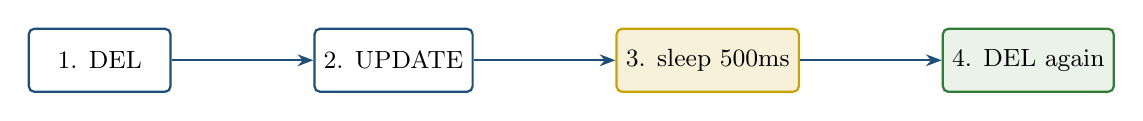
\begin{tikzpicture}[node distance=8mm and 18mm]
  \node[node-box] (s1) {1. DEL};
  \node[node-box,right=of s1] (s2) {2. UPDATE};
  \node[node-box,right=of s2,node-warn] (s3) {3. sleep 500ms};
  \node[node-box,right=of s3,node-ok] (s4) {4. DEL again};
  \draw[arrow] (s1) -- (s2);
  \draw[arrow] (s2) -- (s3);
  \draw[arrow] (s3) -- (s4);
\end{tikzpicture}
\vspace{2mm}
\begin{itemize}
  \item 第一次 DEL 把所有进行中的读"清零"。
  \item UPDATE 写 master。
  \item sleep 覆盖主从延迟 + 并发读"回填脏值"的窗口。
  \item 第二次 DEL 清除可能被脏值回填的缓存。
\end{itemize}
\end{frame}

\begin{frame}{500ms 怎么来的？}
\begin{itemize}
  \item 主从延迟 P99 一般 50--200ms（机房内）。
  \item 业务读耗时 + 网络 RTT 一般 10--100ms。
  \item 500ms 给两者留足冗余 —— 不是公式，是经验值。
  \item 真实系统建议监控主从延迟，动态调整。
\end{itemize}
\vspace{2mm}
\keypoint{延迟双删\textbf{不是}强一致，是"窗口期可控的最终一致"。}
\srcnote{repository/cache/product.go:16 \texttt{ProductDelayInterval = 500 * time.Millisecond}}
\end{frame}

\begin{frame}[fragile]{ProductUpdate 的写路径}
\begin{lstlisting}[language=Go,firstnumber=271,
  caption={\srcnote{service/product.go:271--292}}]
func (s *ProductSrv) ProductUpdate(ctx context.Context, req *types.ProductUpdateReq) (...) {
    product := &model.Product{...}
    _ = cache.DelProductDetail(ctx, req.ID)               // 1. 第一次删
    err = dao.NewProductDao(ctx).UpdateProduct(req.ID, product) // 2. 写 DB
    if err != nil {
        log.LogrusObj.Error(err); return
    }
    cache.DoubleDeleteAsync(req.ID, 0)                    // 3+4. 异步等 500ms 再删
    emitProductChanged(ctx, req.ID, "update")
    return
}
\end{lstlisting}
\end{frame}

\begin{frame}[fragile]{DoubleDeleteAsync 实现}
\begin{lstlisting}[language=Go,firstnumber=64,
  caption={\srcnote{repository/cache/product.go:64--74}}]
// DoubleDeleteAsync: 写库后已经做了第一次删除，这里在 interval 后再删一次，
// 用于覆盖"读旧值的并发请求把旧值塞回缓存"的窗口。
func DoubleDeleteAsync(id uint, interval time.Duration) {
    if interval <= 0 {
        interval = ProductDelayInterval
    }
    go func() {
        time.Sleep(interval)
        _ = RedisClient.Del(context.Background(), ProductDetailKey(id)).Err()
    }()
}
\end{lstlisting}
\vspace{1mm}
\small 用独立 goroutine 异步处理，不阻塞业务返回；第二次 DEL 失败也不影响主路径。
\end{frame}

% ============== 5. 读路径 ==============
\section{读路径的击穿保护}

\begin{frame}{读路径的击穿场景}
\begin{tikzpicture}[node distance=8mm]
  \node[node-box] (req1) {Req 1};
  \node[node-box,below=of req1] (req2) {Req 2};
  \node[node-box,below=of req2] (req3) {... 1000 个 ...};
  \node[node-box,right=22mm of req2] (cache) {Redis};
  \node[node-box,right=22mm of cache,node-bad] (db) {DB};
  \draw[arrow-bad] (req1.east) -- node[above,font=\tiny]{miss} (cache.west);
  \draw[arrow-bad] (req2.east) -- (cache.west);
  \draw[arrow-bad] (req3.east) -- (cache.west);
  \draw[arrow-bad] (cache) -- node[above,font=\tiny]{1000 个回源} (db);
\end{tikzpicture}
\vspace{2mm}
\small 热 key 过期瞬间，所有读全部 miss $\to$ 同时打 DB $\to$ DB 被打挂。
\end{frame}

\begin{frame}{SETNX 回源锁：单飞回源}
\begin{tikzpicture}[node distance=8mm]
  \node[node-box] (req1) {Req 1};
  \node[node-box,below=of req1] (req2) {Req 2};
  \node[node-box,below=of req2] (req3) {Req 3};
  \node[node-box,right=18mm of req2] (lock) {SETNX lock};
  \node[node-box,right=18mm of lock,node-ok] (db) {DB};
  \draw[arrow] (req1.east) -- node[above,font=\tiny]{抢到}(lock);
  \draw[arrow-async] (req2.east) -- node[above,font=\tiny,sloped]{没抢到 sleep 50ms}(lock);
  \draw[arrow-async] (req3.east) -- (lock);
  \draw[arrow] (lock) -- node[above,font=\tiny]{1 个回源} (db);
\end{tikzpicture}
\vspace{2mm}
\small 全局只有一个回源；其他请求 sleep 后重读缓存（多半已经命中）。
\srcnote{repository/cache/product.go:55--62 + service/product.go:42--67}
\end{frame}

\begin{frame}[fragile]{ProductShow Cache Aside + SETNX}
\begin{lstlisting}[language=Go,firstnumber=42,
  caption={\srcnote{service/product.go:42--68}}]
cached := &types.ProductResp{}
if cacheErr := cache.GetProductDetail(ctx, req.ID, cached); cacheErr == nil {
    return cached, nil
}
locked, _ := cache.TryProductLock(ctx, req.ID)
if !locked {
    time.Sleep(50 * time.Millisecond)
    if cacheErr := cache.GetProductDetail(ctx, req.ID, cached); cacheErr == nil {
        return cached, nil
    }
} else {
    defer cache.UnlockProduct(ctx, req.ID)
}
pResp, err := s.loadProductFromDB(ctx, req.ID)
if err != nil { return nil, err }
cache.SetProductDetail(ctx, req.ID, pResp)
return pResp, nil
\end{lstlisting}
\end{frame}

\begin{frame}{为什么不用 Go 的 singleflight}
\begin{itemize}
  \item Go 标准库 \texttt{singleflight} 只在\textbf{单进程内}合并请求。
  \item 服务多实例部署后，每个实例自己 singleflight $\to$ N 个回源同时打 DB。
  \item Redis SETNX 是\textbf{跨进程}的全局锁，才是真正的"全局单飞"。
  \item 短 TTL (3s) 防止锁持有者崩溃导致死锁。
\end{itemize}
\srcnote{repository/cache/product.go:14--17 \texttt{ProductLockTTL = 3 * time.Second}}
\end{frame}

% ============== 6. 终极方案 ==============
\section{binlog 订阅}

\begin{frame}{终极方案：Canal $\to$ MQ $\to$ 异步刷}
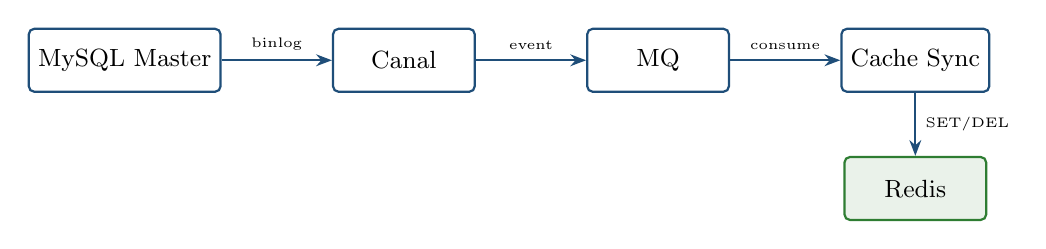
\begin{tikzpicture}[node distance=8mm and 14mm]
  \node[node-box] (master) {MySQL Master};
  \node[node-box,right=of master] (canal) {Canal};
  \node[node-box,right=of canal] (mq) {MQ};
  \node[node-box,right=of mq] (consumer) {Cache Sync};
  \node[node-box,below=of consumer,node-ok] (redis) {Redis};
  \draw[arrow] (master) -- node[above,font=\tiny]{binlog} (canal);
  \draw[arrow] (canal) -- node[above,font=\tiny]{event} (mq);
  \draw[arrow] (mq) -- node[above,font=\tiny]{consume} (consumer);
  \draw[arrow] (consumer) -- node[right,font=\tiny]{SET/DEL} (redis);
\end{tikzpicture}
\vspace{2mm}
\begin{itemize}
  \item 应用层不再负责缓存一致性，binlog 是事实之源。
  \item 收益：业务代码简洁；代价：多一套运维 (Canal/Debezium + MQ)。
\end{itemize}
\end{frame}

\begin{frame}{还有哪些坑}
\begin{itemize}
  \item 删失败要重试 —— 引入"删失败补偿队列"。
  \item 多层缓存 (本地 + Redis) —— 本地缓存的失效要广播。
  \item TTL 雪崩 —— 给 TTL 加随机抖动 (\texttt{ttl + rand[0, 60s]})。
  \item 缓存穿透 —— Bloom Filter / 空值缓存。
\end{itemize}
\srcnote{docs/blog/03-cache-consistency.md \S 还有哪些坑}
\end{frame}

% ============== 7. 性能 ==============
\section{压测数据}

\begin{frame}{大表场景下的真实收益}
\begin{tabular}{@{}lrr@{}}
\toprule
链路 & RPS & p95 \\
\midrule
Ping 基线 & 64{,}254 & 3.51ms \\
商品详情 (DB + PK，未接缓存) & 62{,}226 & 3.01ms \\
商品列表 (DB count 全表，956K 行) & \textbf{24.5} & \textbf{2.50s} \\
\bottomrule
\end{tabular}

\vspace{2mm}
\small \texttt{product/show} 走主键查询，单点延迟和 ping 几乎重合：硬件 cap 在这里。\\
\texttt{product/list} 跌到 \textbf{24.5 RPS / p95 2.5s} —— 瓶颈是 956K 行 \texttt{COUNT(*)} 每次全表扫，正是缓存能挡的工作量。
\srcnote{stressTest/REPORT.md \S 链路压测 第 1/2/8 行（基线 64{,}254 / DB+PK 62{,}226 / count 全表 24.5 RPS）}
\end{frame}

\begin{frame}{游标分页 + 首页缓存：实测 7000$\times$ 吞吐}
\begin{tabular}{@{}lrr@{}}
\toprule
订单列表链路 & RPS & p95 \\
\midrule
旧版深分页 (\texttt{OFFSET 1999999 LIMIT 20}，6M 行) & \textbf{8.3} & \textbf{15.95s} \\
游标分页 + 5min 首页缓存 (PR \#38) & \textbf{58{,}406} & \textbf{5.0ms} \\
\midrule
吞吐比 & \multicolumn{2}{r}{\textbf{$\approx$7{,}000$\times$}} \\
p95 延迟比 & \multicolumn{2}{r}{\textbf{$\approx$3{,}200$\times$}} \\
\bottomrule
\end{tabular}

\vspace{2mm}
\small 优化点有两个：\textbf{游标分页}（\texttt{WHERE id < last\_id LIMIT 20}，PK 倒序 O(1)）+ \textbf{首页 5min Redis 缓存}（Cache Aside）。\\
缓存挡住的不是延迟，是\textbf{DB 全表扫的负载}。这是 Cache Aside 在大表上的真实代差。
\srcnote{stressTest/REPORT.md \S 2. 订单列表 + PR \#38}
\end{frame}

% ============== Q&A ==============
\appendix

\begin{frame}{面试 Q\&A（上）}
\textbf{Q1}：双写一致性的几种方案，各自取舍？\\
\hspace{4mm}\small A：先写后删 / 先删后写都有竞态；延迟双删窗口可控；binlog 异步刷强一致但运维重。

\vspace{2mm}
\textbf{Q2}：延迟双删的"延迟"该设多少？\\
\hspace{4mm}\small A：覆盖主从延迟 + 业务读耗时；本项目 500ms 是经验值，建议监控驱动。

\vspace{2mm}
\textbf{Q3}：缓存击穿和缓存穿透的区别？\\
\hspace{4mm}\small A：击穿是热 key 失效瞬间全打 DB；穿透是查不存在的 key 永远不命中缓存。
\end{frame}

\begin{frame}{面试 Q\&A（下）}
\textbf{Q4}：为什么删不更新缓存？\\
\hspace{4mm}\small A：写双份会引入新的竞态（写顺序），删除是单边操作更鲁棒；下次读会回填。

\vspace{2mm}
\textbf{Q5}：TTL 雪崩怎么避免？\\
\hspace{4mm}\small A：TTL 加随机抖动；热 key 永不过期 + 后台 refresh；多级缓存分散过期时间。

\vspace{2mm}
\textbf{反追问}：本地缓存 (caffeine) 失效广播怎么实现？\\
\hspace{4mm}\small A：用 Redis pub/sub 或 binlog 通道把失效事件广播到所有实例。
\end{frame}

\begin{frame}{代码位置一览}
\begin{description}
  \item[读路径 + SETNX]\srcnote{service/product.go:42--68}
  \item[写路径 + 双删]\srcnote{service/product.go:271--292}
  \item[DoubleDeleteAsync]\srcnote{repository/cache/product.go:64--74}
  \item[TryProductLock / SETNX]\srcnote{repository/cache/product.go:55--62}
  \item[TTL 常量]\srcnote{repository/cache/product.go:14--17}
  \item[压测]\srcnote{stressTest/product\_show.js}
\end{description}
\vspace{2mm}
\keypoint{复现：\texttt{k6 run stressTest/product\_show.js}}
\end{frame}

\end{document}
